\documentclass[../main]{subfiles}
\ifSubfilesClassLoaded{
    \dominitoc
    \tableofcontentsfile
}{}
\begin{document}

\graphicspath{{01-Modularite/},{./}}
%%%%%%%%%%%%%%%%%%%%%%%%%
% Intro du chapitre : Trouver un questionnement, un exemple qui parle de modularité dans les systèmes biologiques:  
% se placer dans le contexte de 
% - modularité : finalement on ne sait pas trop ce que c'est 
% - apprentissage ! 
% - réseaux de neurones
%%%%%%%%%%%%%%%%%%%%%%%%%
\chapter*{Introduction}


Le terme d’intelligence artificielle apparaît en 1956 lors d’une conférence donnée à l’université de Dartmouth, Dartmouth Summer Research Project on Artificial Intelligence. Cette conférence rassemble des chercheurs issus de différents domaines en plein essor de création comme la cybernétique, le traitement de l’information, la logique, la biologie, et veut poser les bases d’un nouveau domaine, nommé à cette occasion par les organisateurs Minsky et McCarthy: “Intelligence artificielle”. 

Ce terme générique est en fait large: on va appeler intelligence artificielle tout programme capable d’effectuer des tâches compliquées dont seuls les humains étaient initialement capables de résoudre. 
En terme d’architectures, les programmes d’intelligence artificielle peuvent être des systèmes figés à base de logique tels que les systèmes experts, ou des systèmes évolutifs. Parmi les tâches dites humaines se trouve en effet la notion d’apprentissage. La création  d’un système apprenant à partir d’entrées devient alors un enjeu à part entière de l’intelligence artificielle qu’on nommera apprentissage automatique ou en anglais machine learning.
Ces 60 dernières années ont alors vu les systèmes “intelligents” évoluer, se diversifier, pour résoudre de plus en plus de tâches jusqu’alors considérées comme humaines.

La conception de ces programmes passe par différentes sources d'inspirations, la biologie y prenant une place de premier choix.

\section*{Conception d'algorithmes d'apprentissage par modularité}

\subsection*{Définition de modularité}

La modularité en informatique se définit comme l'assemblage d'éléments séparés en une fonction globale, avec la condition qu'ajouter ou enlever un element ne modifie pas les autres éléments et influe seulement sur la fonction globale.

La majorité, voir tous les systèmes biologiques peuvent etre compris comme des systèmes modulaires. Il semble d'ailleurs que les systèmes modulaires sont privilégiés par l'évolution et des réseaux de forme similaire se retrouvent ainsi dans de nombreuses branches de la biologie: le cerveau présente des structures de réseau en petit monde que l'on retrouve dans l'organisation des ….
L'ingénieurie, sans même s'inspirer de la nature a recréé ces réseaux: les réseaux small world sont les plus efficaces pour la représentation de bases de données, ou la conception des réseaux aériens.
	
Cette notion de modularité concerne l'informatique en général: le concept peut etre appliqué au développement d'algorithmes.


\subsection*{Conception d'algorithmes d'IA}

La conception d'algorithme passe par piocher dans un ensemble de concepts et de fonctions connues, en les assemblant entre elles. 
La démarche de création d'algorithme peuvent etre ascendantes ou descendantes. 

Exemple d'algos d'IA → 
Ainsi, dans les années 1960, des premiers programmes d'intelligence artificielle repose sur des “micro mondes”, postulant qu'il est plus simple de décomposer les taches en taches plus simples afin de résoudre des comportements plus compliqués.

\subsection*{Approche ascendante vs approche descendantes}

On peut choisir deux axes de recherche pour développer un programme modulaire.
 L'approche descendante, la plus souvent utilisée, part du problème applicatif à résoudre pour le décomposer en probèmes-blocs plus simples.  et on estime que l'assemblage d'éléments exécutant ces fonctions simples nous permettrons d'effectuer la fonction complexe.
Cette démarche est très applicative. Elle est maitrisée: on connait la fonction finale, il suffit de trouver les meilleurs composants pour effectuer cette tache. Généralement, on a de bons résultats
Par contre, on ne pourra pas trouver de nouveaux paradigmes de calculs dans ce cadre: il s’agit plutot d’utiliser et d”appliquer des méthodes connues. 

Dans une démarche ascendante, il s’agit de partir de fonctions simples qu’on assemble dans l’idée d’en créer des complexes. Cette démarche est plutot exploratoire : la complexité du système fait que le seul moyen de comprendre le comportement du système ainsi créé est de le simuler. Cela peut etre vu comme un désavantage: pas possible d’avoir des équations et de choisir correctement les paramètres sans une étude des simulations. L’avantage par contre est de laisser de nombreuses opportunités ouvertes pour de nouvelles formes de calcul.
Et c’est précisément ce point qui nous amène à nous placer dans une telle démarche dans cette thèse. Nous voulons trouver de nouvelles formes de calcul pour faire de l’apprentissage. 

-----

\section*{ Modularité, systèmes complexes et emergence}

Un autre axe motivant notre reflexion sur des architectures modulaires d’apprentissage est l’observation que les systèmes modulaires sont des systèmes complexes. 

\subsection*{Système modulaire = système complexe ? }

Un système complexe est un système dont l'état est décrit par un certain nombre de variables qui évoluent de façon non linéaire. → def de qui ?
Dans la littérature, on rencontre également cette définition: système composé d'un grand nombre d'élements connectés entre eux. Cette définition rejoint la première, mais on peut noter qu'un système peut etre complexe meme à partir de 3 variables, tel que le modèle climatique de Lorentz ou le pendule triple.
 
La complexité d'un système est plutot un mode de représentation du système. La notion de systèmes complexes a été introduite dans les années 70 (Lorenz), et connait un essor depuis l'avenement des calculateur performants. 

Théorie des réseaux complexes

\subsection*{Emergence de calcul au sein d'un système complexe}

On va caractériser l'émergence de comportement dans un système complexe comme “le tout est plus que la somme des parties”, c'est à dire qu'on ne peut pas comprendre un système en le décomposant en éléments et en analysant chaque élémént individuellement: il va falloir considérer les relations entre éléments. 
La notion de systèmes complexe est étroitement liée à celle d'auto-organisation. La présence de patterns réguliers dans le comportement d'un système est directement liée à sa complexité.

\subsection*{Emergence de calcul comme moyen de conception de nouveaux algo d'IA}

D'un point de vue de création de systèmes, cela veut dire qu'on peut construire un système a partir d’éléments séparés, dont le comportement global résulte de l'interaction de ces éléments..
Le deep learning a été construit a partir du perceptron comme un assemblage de couches, dans le but de ????



\section*{ Plan de la thèse}

Dans cette thèse, nous voulons prendre une démarche constructive d'un algorithme d'apprentissage afin d'explorer de nouveaux paradigmes de calcul. Nous explorerons donc un système modulaire donc les modules sont des structures d'apprentissage existantes. Ce modèle dynamique est un système complexe, duquel pourra émerger des comportements
L'émergence de phénomènes d'auto organisation au sein des systèmes complexe nous pousse a considérer des modules possèdant déjà cette capacité d'auto-organisation: les cartes auto-organisatrices de Kohonen.
Le but de cette thèse est ainsi, dans une démarche constructive, de rechercher des nouveaux comportement d'apprentissage  à partir de cartes de Kohenen ,assemblées en architectures.
Nous nous intéressons à des modèles décentralisés, étant la clé pour construire n'importe quel type d'architecture par la suite. 
Cette démarche est difficile dans la mesure ou le comportement final d'une architecture n'est pas prédictible de prime abord. Tout l'exercice de cette thèse est alors de construire un modèle et définir des règles d'interaction, puis simuler et analyser ce modèle pour en tirer des comportements émergeants participant à l'apprentissage.
Dans cette démarche de construction, nous avons choisi des contraintes:
- Nous réalisons un système modulaire de cartes auto-organisatrices
- Cette architecture sera décentralisée: nous voulons permettre aux modules de communiquer avec n'importe lequel des autres éléments.
Le problème de cette thèse est d'étudier les comportements émergent de tels systèmes et d'étudier comment ces comportements sont un apprentissage des données.
Nous comparerons dans un premier chapitre les systèmes de cartes auto-organisatrices présentes dans la littérature et positionnerons l'architecture que nous développerons dans ce manuscrit au regard des travaux existants. Ces travaux nous permetterons de poser des hypothèses concernant le comportement qu'on peut attendre de l'architecture que nous développons. Nous présenterons ensuite le modèle CxSOM.
Nous définirons dans un chapitre la démarche expérimentale utilisée pour évaluer l'architecture de cartes et la représenter. Enfin, nous montrerons des comportements de base emergeant de la structure que nous avons développée et montrerons qu'elle a un capacité de mémoire associative. Nous présenterons egalement les limites du modèle. 
A l'issue du manuscrit, nous souhaitons que le lecteur aie une compréhension des comportements de base du modèle proposé, et aie des pistes pour l'utiliser de façon plus applicative.
\begin{figure}
    \begin{minipage}{0.49\textwidth}
        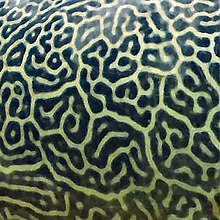
\includegraphics[width=\textwidth]{220px-Giant_Pufferfish_skin_pattern_detail}
    \end{minipage}
    \begin{minipage}{0.49\textwidth}
        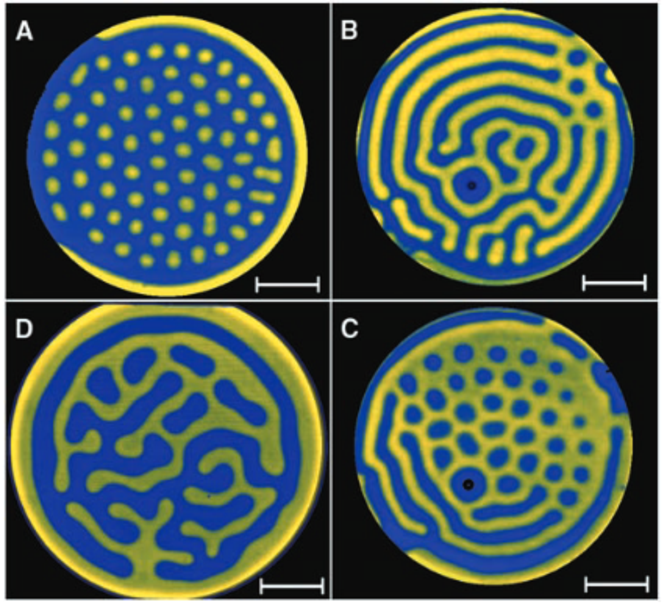
\includegraphics[width=\textwidth]{turing_pattern_chem.pdf}
    \end{minipage}
\end{figure}
\end{document}






